% !TEX encoding = UTF-8
%Koma article
\documentclass[fontsize=12pt,paper=letter,twoside]{scrartcl}
\usepackage{float}
\usepackage{listings}
\usepackage{makecell}

%Standard Pre-amble
\usepackage[top=4cm,bottom=4cm,left=3cm,right=3cm,asymmetric]{geometry}
%\geometry{landscape}                % Activate for for rotated page geometry
%\usepackage[parfill]{parskip}    % Begin paragraphs with an empty line rather than an indent
\usepackage[table,xcdraw]{xcolor}
\usepackage{graphicx}

\usepackage{amsmath}
\usepackage{amssymb}
\usepackage{epstopdf}
\DeclareGraphicsRule{.tif}{png}{.png}{`convert #1 `dirname #1`/`basename #1 .tif`.png}
% Listings needs package courier
\usepackage{listings} % Needs 
\usepackage{courier}

\usepackage[framemethod=TikZ]{mdframed}
\usepackage{url}

\usepackage{sty/bsymb} %% Event-B symbols
\usepackage{sty/eventB} %% REQ and ENV
\usepackage{sty/calculation}

%Maths
\usepackage{amssymb,amsmath}
\def\Fl{\mathbb{F}}
\def\Rl{\mathbb{R}}
\def\Nl{\mathbb{N}}
\def\Bl{\mathbb{B}}
\def\St{\mathbb{S}}
\newcommand{\ovr}{\upharpoonright}
\newcommand{\var}[1]{\textit{#1}}
%Useful definitions
\newcommand{\mv}[1]{\textit{m\_#1}}
\newcommand{\cv}[1]{\textit{c\_#1}}
\newcommand{\degree}[1]{^{\circ}\mathrm{#1}}
%\newcommand{\comment}[1]{{\footnotesize \quad\texttt{--}\textrm{#1}}}
\newcommand{\im}[1]{i\texttt{-\!#1}}

\usepackage[headsepline]{scrpage2}
\pagestyle{scrheadings}
\ihead[]{\small EECS4312 Report1}
\ohead[]{\small \thepage}
\cfoot[]{}
\ofoot[]{}


%%%%PVS environment%%%%%%%%%%%%%%%%%%%
\lstnewenvironment{pvs}[1][]
    {\lstset{#1,captionpos=b,language=pvs,
    mathescape=true,
    basicstyle=\small\ttfamily,
    numbers=none,
    frame=single,
    % numberstyle=\tiny\color{gray},
    % backgroundcolor=\color{lightgray},
    firstnumber=auto
    }}
    {}
 %%%%%%%%%%%%%%%%%%%%%%%%%%%%%%%%
 
%%%%Verbatim environment%%%%%%%%%%%%%%%%%%%
\lstnewenvironment{code}[1][]
    {\lstset{#1,captionpos=b,
    mathescape=true,
    basicstyle=\small\ttfamily,
    numbers=none,
    frame=single,
    % numberstyle=\tiny\color{gray},
    % backgroundcolor=\color{lightgray},
    firstnumber=auto
    }}
    {}

% \newenvironment{boxed}[1]
%    {\begin{center}
%    #1\\[1ex]
%    \begin{tabular}{|p{0.9\textwidth}|}
%    \hline\\
%    }
%    { 
%    \\\\\hline
%    \end{tabular} 
%    \end{center}
%    }
 %%%%%%%%%%%%%%%%%%%%%%%%%%%%%%%%
 
 %Text in a box
\newenvironment{textbox}
    {\begin{center}
    \begin{tabular}{|p{0.9\textwidth}|}
    \hline\\
    }
    { 
    \\\\\hline
    \end{tabular} 
    \end{center}
    }

\usepackage{hyperref}

%Highlight \hl{}
\usepackage{soul}

\usepackage{enumitem}
\newlist{mylist}{itemize}{1}
\setlist[mylist]{label=\textbullet,leftmargin=1cm,nosep}

\usepackage{multirow}

% Reduce space between figure and caption
%\usepackage{caption}
%\captionsetup[table]{font=small,skip=0pt}     %% Adjust here
%or equivalently 
\usepackage[font=small,skip=4pt]{caption}
%Useful definitions
%\newcommand{\mv}[1]{\textit{m\_#1}}
%\newcommand{\cv}[1]{\textit{c\_#1}}
%\newcommand{\degree}[1]{^{\circ}\mathrm{#1}}
%\newcommand{\comment}[1]{{\footnotesize \quad\texttt{--}\textrm{#1}}}


%For Code Stylings
\usepackage{listings}
\usepackage{color}

\definecolor{dkgreen}{rgb}{0,0.6,0}
\definecolor{gray}{rgb}{0.5,0.5,0.5}
\definecolor{mauve}{rgb}{0.58,0,0.82}

\lstset{frame=tb,
  language=Java,
  aboveskip=3mm,
  belowskip=3mm,
  showstringspaces=false,
  columns=flexible,
  basicstyle={\small\ttfamily},
  numbers=none,
  numberstyle=\tiny\color{gray},
  keywordstyle=\color{blue},
  commentstyle=\color{dkgreen},
  stringstyle=\color{mauve},
  breaklines=true,
  breakatwhitespace=true,
  tabsize=3
}

% Set the header
\ihead[]{\small EECS4313 Assignment-3}


%%%%%%%%%%%%Enter your names here%%%%%%%%
\author{Student Name | Student Number | EECS Account
\and \textbf{Edward Vaisman | 212849857 | eddyv}
\and \textbf{Robin Bandzar | 212200531 | cse23028}
\and \textbf{Kirusanth Thiruchelvam | 212918298 | kirusant}
\and \textbf{Sadman Sakib Hasan | 212497509 | cse23152}
}
%%%%%%%%%%%%%%%%%%%%%%%%%%%%%%%%

\date{\today} % Display a given date or no date

\begin{document}
\title{EECS 4313 Assignment 3 \\Data Flow Testing, Slice-Based Testing and Mutation Testing}
\maketitle

\newpage

%%%%%%%%%%%%%%%%%%%%%%%%%%%%%%%
\tableofcontents


\newpage


\section{BORG Calendar}
\subsection{Slice Testing}

\subsubsection{Chosen Method for Testing}

\begin{itemize}
\item \textbf{Class}: \emph{net.sf.borg.common.DateUtil.java}
\item \textbf{Method}: \emph{minuteString(int mins)}
\item \textbf{Method Description}:
This method generate a human reable string for a particular number of minutes. It returns the string in terms of hours or minutes or both hours and mintues.
\begin{itemize}
\item \textbf{mins} - The first argument is of type integer.
\end{itemize}
\end{itemize}

\noindent Following is the code of the \emph{minuteString} method:
\begin{lstlisting}[numbers=left,firstnumber=100]
  public static String minuteString(int mins) {
    
    int hours = mins / 60;
    int minsPast = mins % 60;
    
    String minutesString;
    String hoursString;
    
    if (hours > 1) {
      hoursString = hours + " " + Resource.getResourceString("Hours");
    } else if (hours > 0) {
      hoursString = hours + " " + Resource.getResourceString("Hour");
    } else {
      hoursString = "";
    }

    if (minsPast > 1) {
      minutesString = minsPast + " " + Resource.getResourceString("Minutes");
    } else if (minsPast > 0) {
      minutesString = minsPast + " " + Resource.getResourceString("Minute");
    } else if (hours >= 1) {
      minutesString = "";
    } else {
      minutesString = minsPast + " " + Resource.getResourceString("Minutes");
    }

    // space between hours and minutes
    if (!hoursString.equals("") && !minutesString.equals(""))
      minutesString = " " + minutesString;

    return hoursString + minutesString;
  }
\end{lstlisting}

\subsubsection{Forward Slicing}

The forward slicing is one of the static program slicing. The forward slicing of a program  can be defined in the form of S(v,n)  which refers to all the program statments that are affected by the value of v at statement n. In other words, what staments will be affected in the program by modifying the selected varible's value at the selected statment. The Borg Calendar has two cases where we can apply the forward slice-based testing.
\newline
\\ \textbf {Case 1}: S (hours, 102) -  modifying value of  the variable \emph{hours} at statment 102
\newline
\newline
 In this case, we cannot slice any statment of the program since all of them are depend on variable \emph{hours}. We have two  nested if-else statments and both of them uses variable \emph{hours} in their esle if condition. This makes other conditons on the nested if-else struture to be depend upon the variable of \emph{hour} to execute the program but the value of it would not affect them. Since there is a need for return statment to exeute the code, we cannot slice that statment as well. In order to produce the correct spaces in the outputs we need the if condion made for hourstring and minutes string at statment 127.
 
However, we only need four testcases here to identify how the chage in value of hour affectes the program since other statments in the code do not depend on the vlaue at all and they merely depend on the varible to execute the program successfully due the structure of nested if-else.
 
The following figure show which statments in the method affected by changing value of hours. 
 \begin{figure}[!htb]
\begin{center}
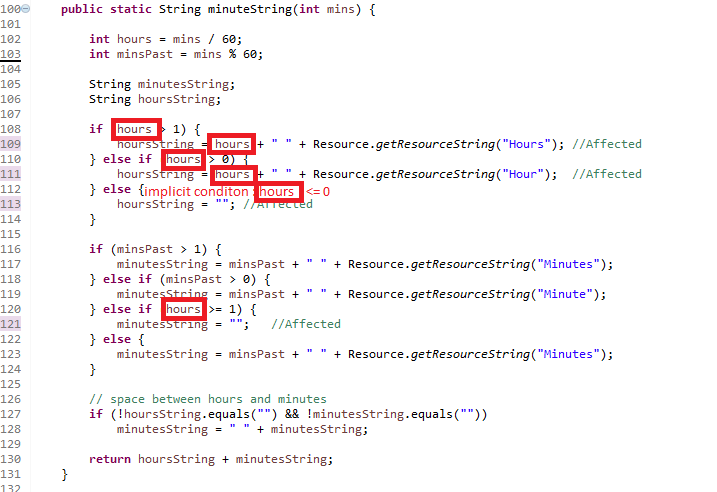
\includegraphics[width=.99\textwidth]{images/forward/hour.png}
\end{center}
\caption{Affected lines due to change in the value of  variable \emph{hours}}
\label{fig:minuteStringCode}
\end{figure}
\newline
\newline
\newline
\newline
In order to check the affected four lines we have implemented threer test cases :
\begin{enumerate}
\item assertEquals("3 Hours",DateUtil.minuteString(180))  - checks staments 108- 109 and statments 120 -121
\item assertEquals("1 Hour",DateUtil.minuteString(60))  - checks statments 110 - 111 and statments 120 -121
\item assertEquals("0 Minutes",DateUtil.minuteString(0)) - checks statments 110 - 111
\end{enumerate}

Since the cases provide full coverage of the affected lines, we only need to consider changing those lines to produce the correct result when we modify the vairable \emph{hours}
\newline
\newline
\textbf {Case 2}: S (minsPast, 103) -  modifying value of  the variable \emph{minsPast} at statment 103

 




 

 

 










\begin{itemize}
\item The data flow analysis you performed and the calculation of the coverage metrics. You must
show which test cases are responsible for which dc-paths.
\item A description of the test cases you added to improve coverage. If your coverage was already high,
discuss how your testing was able to achieve this.
\item The slices that you identified and the percentage of slices that your testing covers. You must
show which test cases are responsible for which slices.
\item A description of the test cases you added to improve slice coverage. If your coverage was
already high, discuss how your testing was able to achieve this.
\item Evaluate the effectiveness of your test cases using mutation testing. Discuss and address any
issues if you have found in your written report.
\item Attaching bug reports if bugs are discovered using your testing methods. You should use the
same bug report format as in Assignment 1. Do not file these bug reports to the project’s bug
report system.
\item An appendix with the specification of the methods you are testing
\end{itemize}

\section{JPetStore}

\begin{itemize}
\item The test scenarios that you have created;
\item The request rates and the duration of the load tests;
\item The analysis of your load tests and the description of any problems that you have found (if there
are any).
\end{itemize}

\end{document}
